% WattPrint -- NILMFormer reproduction and multi-dataset extension.
% Build: `make paper` (from nilmformer-experiment/) or upload this folder to Overleaf.
% Every number in the text is a macro from tables/numbers.tex, generated from data/*.csv by
% scripts/make_figures.py: re-run `make paper-data paper-figures` after any retraining.
\documentclass[conference]{IEEEtran}
\usepackage[T1]{fontenc}
\usepackage[utf8]{inputenc}
\usepackage{amsmath,amssymb}
\usepackage{graphicx}
\usepackage{booktabs}
\usepackage{siunitx}
\usepackage{xcolor}
\usepackage{tikz}
\usetikzlibrary{positioning,arrows.meta,fit}
\usepackage[hidelinks]{hyperref}
\usepackage{cite}
\sisetup{group-separator={,}, group-minimum-digits=4}
\graphicspath{{figures/}}
% generated by paper/scripts/make_figures.py -- do not edit
\newcommand{\KettleFone}{0.835}
\newcommand{\KettleMR}{0.631}
\newcommand{\KettleMAE}{10.3}
\newcommand{\KettleSAE}{0.00}
\newcommand{\KettlePrec}{0.802}
\newcommand{\KettleRec}{0.872}
\newcommand{\KettleTrueKWh}{224}
\newcommand{\KettlePredKWh}{224}
\newcommand{\MWFone}{0.236}
\newcommand{\MWMR}{0.071}
\newcommand{\MWMAE}{4.9}
\newcommand{\MWSAE}{0.61}
\newcommand{\MWPrec}{0.208}
\newcommand{\MWRec}{0.274}
\newcommand{\MWTrueKWh}{29}
\newcommand{\MWPredKWh}{11}
\newcommand{\DWFone}{0.802}
\newcommand{\DWMR}{0.475}
\newcommand{\DWMAE}{42.8}
\newcommand{\DWSAE}{0.22}
\newcommand{\DWPrec}{0.753}
\newcommand{\DWRec}{0.857}
\newcommand{\DWTrueKWh}{611}
\newcommand{\DWPredKWh}{477}
\newcommand{\WMRefitFone}{0.443}
\newcommand{\WMRefitMR}{0.115}
\newcommand{\WMRefitMAE}{20.0}
\newcommand{\WMRefitSAE}{0.82}
\newcommand{\WMRefitPrec}{0.564}
\newcommand{\WMRefitRec}{0.365}
\newcommand{\WMRefitTrueKWh}{187}
\newcommand{\WMRefitPredKWh}{33}
\newcommand{\FridgeRefitFone}{0.768}
\newcommand{\FridgeRefitMR}{0.521}
\newcommand{\FridgeRefitMAE}{22.3}
\newcommand{\FridgeRefitSAE}{0.21}
\newcommand{\FridgeRefitPrec}{0.762}
\newcommand{\FridgeRefitRec}{0.774}
\newcommand{\FridgeRefitTrueKWh}{372}
\newcommand{\FridgeRefitPredKWh}{294}
\newcommand{\TDFone}{0.813}
\newcommand{\TDMR}{0.353}
\newcommand{\TDMAE}{10.0}
\newcommand{\TDSAE}{0.40}
\newcommand{\TDPrec}{0.692}
\newcommand{\TDRec}{0.985}
\newcommand{\TDTrueKWh}{121}
\newcommand{\TDPredKWh}{72}
\newcommand{\ACFone}{0.809}
\newcommand{\ACMR}{0.426}
\newcommand{\ACMAE}{89.7}
\newcommand{\ACSAE}{0.41}
\newcommand{\ACPrec}{0.939}
\newcommand{\ACRec}{0.711}
\newcommand{\ACTrueKWh}{1{,}446}
\newcommand{\ACPredKWh}{857}
\newcommand{\WHFone}{0.985}
\newcommand{\WHMR}{0.886}
\newcommand{\WHMAE}{7.8}
\newcommand{\WHSAE}{0.06}
\newcommand{\WHPrec}{0.981}
\newcommand{\WHRec}{0.988}
\newcommand{\WHTrueKWh}{638}
\newcommand{\WHPredKWh}{602}
\newcommand{\FridgeFone}{0.801}
\newcommand{\FridgeMR}{0.612}
\newcommand{\FridgeMAE}{17.2}
\newcommand{\FridgeSAE}{0.42}
\newcommand{\FridgePrec}{0.880}
\newcommand{\FridgeRec}{0.735}
\newcommand{\FridgeTrueKWh}{417}
\newcommand{\FridgePredKWh}{241}
\newcommand{\WMFone}{0.468}
\newcommand{\WMMR}{0.229}
\newcommand{\WMMAE}{4.7}
\newcommand{\WMSAE}{0.16}
\newcommand{\WMPrec}{0.409}
\newcommand{\WMRec}{0.546}
\newcommand{\WMTrueKWh}{39}
\newcommand{\WMPredKWh}{32}
\newcommand{\HouseMeanFone}{0.77}
\newcommand{\HouseKWh}{3{,}135}
\newcommand{\HouseDays}{427}
\newcommand{\HouseMissing}{3.6}
\newcommand{\HouseMetered}{81}
\newcommand{\HouseFound}{69}
\newcommand{\NParams}{383{,}283}
\newcommand{\ACTrueShare}{46}
\newcommand{\ACPredShare}{28}
\newcommand{\WHTrueShare}{20}
\newcommand{\WHPredShare}{19}
\newcommand{\FridgeTrueShare}{13}
\newcommand{\FridgePredShare}{8}
\newcommand{\WMTrueShare}{1}
\newcommand{\WMPredShare}{1}
\newcommand{\OtherTrueShare}{19}
\newcommand{\OtherPredShare}{44}
\newcommand{\ACJulTrue}{429}
\newcommand{\ACJulPred}{360}
\newcommand{\ACJulPct}{84}
\newcommand{\ACJanTrue}{166}
\newcommand{\ACJanPred}{59}
\newcommand{\ACJanPct}{36}
\newcommand{\ACQfourF}{0.476}
\newcommand{\ACQthreeF}{0.874}
\newcommand{\FridgeThrTunedFone}{0.148}
\newcommand{\FridgeThrTunedSAE}{0.82}
\newcommand{\FridgeThrTunedMRpp}{0.079}
\newcommand{\FridgeThrTunedThr}{92}
\newcommand{\FridgeThrFixedFone}{0.801}
\newcommand{\FridgeThrFixedSAE}{0.42}
\newcommand{\FridgeThrFixedMRpp}{0.527}
\newcommand{\FridgeThrFixedThr}{20}
\newcommand{\FridgeRefitOnlyFone}{0.875}
\newcommand{\FridgeRefitOnlySAE}{0.45}
\newcommand{\FridgeRefitOnlyMRpp}{0.461}
\newcommand{\FridgeRefitOnlyThr}{20}
\newcommand{\WMRefitOnlyFone}{0.333}
\newcommand{\WMRefitOnlySAE}{0.27}
\newcommand{\WMRefitOnlyMRpp}{0.178}
\newcommand{\WMRefitOnlyThr}{111}
\newcommand{\FridgeRefitPlegmaFone}{0.801}
\newcommand{\FridgeRefitPlegmaSAE}{0.42}
\newcommand{\FridgeRefitPlegmaMRpp}{0.525}
\newcommand{\FridgeRefitPlegmaThr}{20}
\newcommand{\FridgeConstDays}{68}
\newcommand{\FridgeConstW}{72}
\newcommand{\FridgeExclFone}{0.913}
\newcommand{\FridgeExclSAE}{0.25}
\newcommand{\FridgeDailyRall}{0.13}
\newcommand{\FridgeDailyRexcl}{0.90}
\newcommand{\TDFalseKWh}{120}


\begin{document}

\title{Reproducing NILMFormer and Extending It to Air Conditioners and Water Heaters\\with Multi-Dataset Training}

\author{\IEEEauthorblockN{[Authors]}
\IEEEauthorblockA{{[Affiliation]} \\ {[email]}}}

\maketitle

\begin{abstract}
Non-intrusive load monitoring (NILM) estimates the consumption of individual appliances from a
single household meter. We reproduce NILMFormer, a 0.385M-parameter Transformer for
sequence-to-sequence NILM, under the training protocol of its paper on the REFIT dataset, and
extend it to the appliances that dominate consumption in warm climates. REFIT has neither air
conditioners (AC) nor electric water heaters, so we harmonise two further public datasets, Plegma
(Greece) and PRECON (Pakistan), into the REFIT layout and train eight appliance models with an
unchanged pipeline. On REFIT, our matching ratio exceeds the published one for kettle and
dishwasher (\KettleMR{} and \DWMR{}) and falls short for microwave and washing machine. On a
Plegma household held out from every model, covering \HouseDays{} days and \HouseKWh{}~kWh, the
system reaches an F1 of \WHFone{} for the water heater, \ACFone{} for the AC, \FridgeFone{} for
the fridge and \WMFone{} for the washing machine. The AC is detected reliably (precision
\ACPrec{}) but its energy is under-estimated, mostly in heating mode. Ablations show that a
cycling-load threshold tuned on another house can collapse the fridge F1 from \FridgeThrFixedFone{}
to \FridgeThrTunedFone{}, and that \FridgeConstDays{} days of non-cycling fridge consumption are
invisible to any NILM model.
\end{abstract}

\begin{IEEEkeywords}
Non-intrusive load monitoring, energy disaggregation, Transformer, air conditioning, transfer across datasets
\end{IEEEkeywords}

% =============================================================================================
\section{Introduction}
Appliance-level feedback helps households cut their electricity use, but sub-metering every
appliance is costly. NILM~\cite{hart1992nilm} infers it from the aggregate signal of one meter.
Deep sequence models~\cite{kelly2015neuralnilm,zhang2018seq2point,yue2020bert4nilm} are now the
standard approach, and NILMFormer~\cite{petralia2025nilmformer} reports state-of-the-art accuracy
at low sampling rates (1~min) with a small model that is deployed at national scale.

Published NILM benchmarks are dominated by UK datasets~\cite{murray2017refit,kelly2015ukdale},
whose appliance set (kettle, microwave, dishwasher, washing machine) does not match the loads that
dominate bills in hot climates: air conditioners and electric water heaters. Our target
deployment is a Vietnamese household energy service, for which no public sub-metered dataset
with AC exists. This paper reports:
\begin{itemize}
  \item a reproduction of NILMFormer on REFIT under the paper's protocol, compared to the
        published numbers (Sec.~\ref{sec:repro});
  \item a harmonisation of Plegma~\cite{athanasoulias2024plegma} and PRECON~\cite{nadeem2019precon}
        into the REFIT layout, which lets the unmodified pipeline train AC, water-heater, fridge
        and tumble-dryer models (Sec.~\ref{sec:data});
  \item a detailed evaluation on one held-out household, which is the one served by our backend,
        with ablations on training data and post-processing (Sec.~\ref{sec:house}).
\end{itemize}

% =============================================================================================
\section{Model}\label{sec:model}
NILMFormer maps a window of $L=128$ aggregate samples to $L$ samples of one appliance's power,
with one model per appliance (Fig.~\ref{fig:arch}). Two components address the non-stationarity
of load curves.

\textbf{Subsequence stationarisation.} Each input window is normalised by its own mean $\mu$ and
standard deviation $\sigma$. The pair $(\mu,\sigma)$ is projected into a token that is appended to
the sequence. After the encoder, that token is projected back to the mean and standard deviation of
the \emph{output}, which de-normalises the prediction. This differs from RevIN~\cite{kim2022revin},
which re-applies the input statistics.

\textbf{TimeRPE.} Minute, hour, day of week and month of each sample are encoded with sine and
cosine (8 channels) and projected by a $1{\times}1$ convolution to $d/4$ channels. They are
concatenated with a dilated residual convolution embedding of the load curve ($3d/4$ channels,
dilations 1, 2, 4, 8).

The encoder has 3 Transformer layers ($d=96$, 8 heads, FFN ratio 4, dropout 0.2) with a
diagonally masked self-attention, followed by a convolutional head. The model has \NParams{}
parameters, versus 0.385M in the paper.

\begin{figure}[t]
\centering
\resizebox{\columnwidth}{!}{%
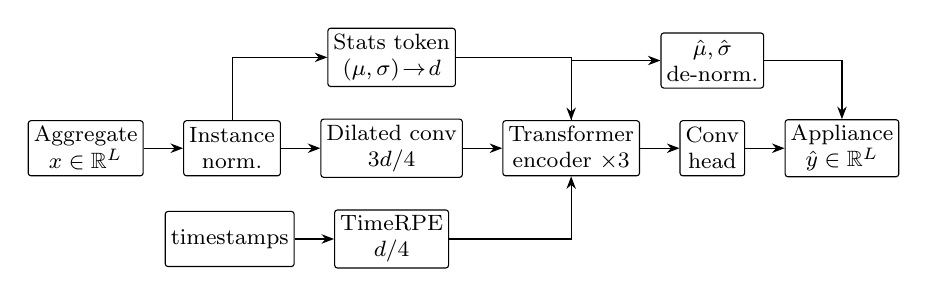
\begin{tikzpicture}[node distance=4mm and 5mm, every node/.style={font=\footnotesize},
  box/.style={draw, rounded corners=1pt, align=center, minimum height=7mm, inner sep=2pt},
  arr/.style={-{Stealth[length=1.6mm]}}]
  \node[box] (x) {Aggregate\\$x\in\mathbb{R}^{L}$};
  \node[box, right=of x] (norm) {Instance\\norm.};
  \node[box, right=of norm] (emb) {Dilated conv\\$3d/4$};
  \node[box, below=of emb] (time) {TimeRPE\\$d/4$};
  \node[box, left=of time] (ts) {timestamps};
  \node[box, above=of emb] (stat) {Stats token\\$(\mu,\sigma)\!\to\!d$};
  \node[box, right=of emb] (enc) {Transformer\\encoder $\times3$};
  \node[box, right=of enc] (head) {Conv\\head};
  \node[box, right=of head] (y) {Appliance\\$\hat y\in\mathbb{R}^{L}$};
  \node[box, above=of head] (denorm) {$\hat\mu,\hat\sigma$\\de-norm.};
  \draw[arr] (x) -- (norm); \draw[arr] (norm) -- (emb); \draw[arr] (emb) -- (enc);
  \draw[arr] (ts) -- (time); \draw[arr] (time) -| (enc);
  \draw[arr] (norm) |- (stat); \draw[arr] (stat) -| (enc);
  \draw[arr] (enc) -- (head); \draw[arr] (head) -- (y);
  \draw[arr] (enc.north) |- (denorm); \draw[arr] (denorm) -| (y);
\end{tikzpicture}}
\caption{NILMFormer~\cite{petralia2025nilmformer}. The statistics token carries the input scale
through the encoder and predicts the output scale.}
\label{fig:arch}
\end{figure}

% =============================================================================================
\section{Data}\label{sec:data}
\subsection{Datasets}
\textbf{REFIT}~\cite{murray2017refit}: 20 UK houses, 2013--2015, aggregate and 9 appliance plugs
at about 8~s (CC BY 4.0). It is the dataset of the paper's REFIT results.
\textbf{Plegma}~\cite{athanasoulias2024plegma}: 13 Greek houses, 2022--2023, 10~s plug-level
measurements including AC units and electric water heaters (CC BY 4.0).
\textbf{PRECON}~\cite{nadeem2019precon}: 42 houses in Lahore, Pakistan, June 2018--May 2019, 1~min
\emph{circuit}-level measurements; no licence is stated, so we use it for research only.
We found no public sub-metered dataset with AC for Vietnam or South-East Asia.

\subsection{Harmonisation}
A converter writes each Plegma and PRECON house as a REFIT \texttt{CLEAN\_House} file (time,
aggregate, appliance channels in W, issue flag) with a \texttt{HOUSES\_Labels} entry, so that the
original REFIT data builder reads it unchanged. House identifiers are offset per dataset (REFIT
1--21, Plegma 101--113, PRECON 201--242). Several units of one type (multiple ACs, two fridges)
are summed, and a minute is missing as soon as one unit is. For PRECON we drop the
\texttt{AC\_UPS} circuits, which mix the AC with UPS-backed loads. We keep only the 6 houses in
which \emph{every} AC is metered, as reported in the metadata; otherwise the unmetered units would
remain unlabelled in the aggregate. Minutes with a missing or non-positive aggregate are flagged as
issues.

\subsection{Preprocessing and splits}
The REFIT builder resamples to 10~s, forward-fills gaps of up to 90~s, zeroes values below 5~W,
clips at 10~kW, derives ON states from per-appliance thresholds and averages to 1~min.
Training uses non-overlapping windows of 128~min. The scaler is fitted on the training houses
only. Table~\ref{tab:splits} lists the houses of each model. The paper appliances keep the paper's
house lists, with REFIT house~2 for test and house~9 for validation. The models served to the
backend are tested on Plegma~101 and validated on Plegma~103, and both houses are excluded from
the training of every model.

\begin{table}[t]
\centering\footnotesize\setlength{\tabcolsep}{3pt}
\caption{Training houses per model (count per dataset), validation and test house.}
\label{tab:splits}
\resizebox{\columnwidth}{!}{% generated by paper/scripts/make_figures.py -- do not edit
\begin{tabular}{@{}llrrrrr@{}}
\toprule
Model & Training data & REFIT & Plegma & PRECON & Valid & Test \\
\midrule
Kettle & REFIT & 10 & 0 & 0 & 9 & 2 \\
Microwave & REFIT & 12 & 0 & 0 & 9 & 2 \\
Dishwasher & REFIT & 11 & 0 & 0 & 9 & 2 \\
Washing machine (REFIT only) & REFIT & 13 & 0 & 0 & 9 & 2 \\
Washing machine & REFIT + Plegma & 15 & 11 & 0 & 103 & 101 \\
Fridge (REFIT only) & REFIT & 5 & 0 & 0 & 9 & 2 \\
Fridge & REFIT + Plegma & 7 & 11 & 0 & 103 & 101 \\
Tumble dryer & REFIT & 7 & 0 & 0 & 13 & 15 \\
Air conditioner & Plegma + PRECON & 0 & 9 & 6 & 103 & 101 \\
Water heater & Plegma & 0 & 10 & 0 & 103 & 101 \\
\bottomrule
\end{tabular}
}
\end{table}

% =============================================================================================
\section{Training and Inference Pipeline}\label{sec:pipeline}
\textbf{Protocol.} As in the paper: up to 50 epochs, early stopping with patience 10 (the best
weights are restored), ReduceLROnPlateau with patience 5, batch 64, AdamW (no weight decay) with
lr $10^{-4}$, and MSE loss. Deviations: one validation and one test house instead of two test
houses, shuffled training batches, and a single seed instead of three.

\textbf{Post-processing.} The raw output is median-smoothed, thresholded and stripped of ON runs
shorter than a minimum length. The threshold is chosen for F1 on the validation house, except for
the fridge (Sec.~\ref{sec:ablation}). An energy gain $g=\mathrm{clip}(E_\text{true}/E_\text{pred},
0.5, 3)$, measured on the validation house, compensates the MSE models' tendency to shrink the ON
level. The appliance sum is capped by the aggregate and the remainder is reported as ``Other''.
Models run only for appliances the household owns (\emph{inventory}).

\textbf{Inference.} One RTX~5880 Ada GPU trains several models in parallel, each in
6--23~min (Table~\ref{tab:training}). An HTTP service applies the same code path as offline
prediction, with overlapping windows averaged, and answers a 256-minute request in about 7~ms.

\begin{table}[t]
\centering\footnotesize
\caption{Training runs: epochs until early stopping, best epoch, best validation loss (MSE on
scaled data, not comparable across appliances) and training time. R: REFIT only; R+P: REFIT and Plegma.}
\label{tab:training}
% generated by paper/scripts/make_figures.py -- do not edit
\begin{tabular}{@{}lrrrr@{}}
\toprule
Model & Epochs & Best & Best valid loss & Train time (min) \\
\midrule
Kettle & 21 & 11 & \num{1.17e-04} & 17.1 \\
Microwave & 13 & 3 & \num{1.61e-05} & 13.2 \\
Dishwasher & 15 & 5 & \num{4.21e-04} & 14.1 \\
Washing machine (R) & 17 & 7 & \num{1.71e-04} & -- \\
Washing machine (R+P) & 20 & 10 & \num{5.99e-05} & 23.3 \\
Fridge (R) & 15 & 5 & \num{2.66e-05} & -- \\
Fridge (R+P) & 29 & 19 & \num{3.93e-06} & 21.0 \\
Tumble dryer & 13 & 1 & \num{8.29e-04} & 6.6 \\
Air conditioner & 15 & 5 & \num{2.99e-04} & 9.6 \\
Water heater & 22 & 12 & \num{3.12e-04} & 8.1 \\
\bottomrule
\end{tabular}

\end{table}

\begin{figure*}[t]
\centering
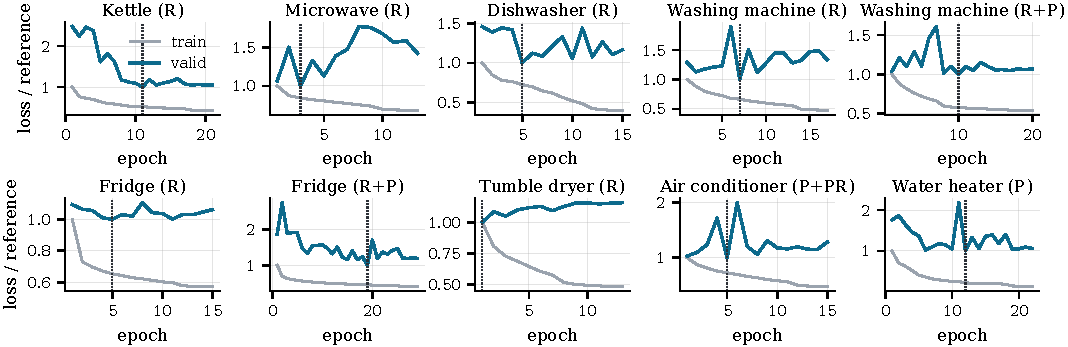
\includegraphics[width=\textwidth]{training_curves}
\caption{Training curves, normalised by the first training loss and by the best validation loss.
The dotted line marks the restored epoch. R: REFIT, P: Plegma, PR: PRECON.}
\label{fig:curves}
\end{figure*}

% =============================================================================================
\section{Results}
\subsection{Reproduction on REFIT}\label{sec:repro}
Table~\ref{tab:paper} and Fig.~\ref{fig:paper} compare our raw predictions with the paper's
REFIT results at 1~min and $w=128$, using the paper's metrics: MAE and the matching ratio
$\mathrm{MR}=\sum_t\min(\hat y_t,y_t)/\sum_t\max(\hat y_t,y_t)$. Our MR is higher for kettle
(\KettleMR{} vs 0.522) and dishwasher (\DWMR{} vs 0.332), and lower for microwave (\MWMR{} vs
0.110) and washing machine (\WMRefitMR{} vs 0.250). The setting differs: the paper averages two test
houses and three seeds, while we use one of each. MAE scales with how much the test house uses the
appliance, which explains our higher dishwasher MAE despite the better MR. The microwave, short and
low-power, remains the hardest case, as in the paper.

\begin{table}[t]
\centering\footnotesize
\caption{REFIT, 1~min, $w=128$. Paper: NILMFormer, Table~2 of~\cite{petralia2025nilmformer}.
Ours: REFIT house~2, raw output; F1 after post-processing (not reported by the paper).}
\label{tab:paper}
% generated by paper/scripts/make_figures.py -- do not edit
\begin{tabular}{@{}lrrrrr@{}}
\toprule
 & \multicolumn{2}{c}{MAE (W) $\downarrow$} & \multicolumn{2}{c}{MR $\uparrow$} & F1 $\uparrow$ \\
\cmidrule(lr){2-3}\cmidrule(lr){4-5}\cmidrule(l){6-6}
Appliance & Paper & Ours & Paper & Ours & Ours \\
\midrule
Kettle & \textbf{9.3} & 10.3 & 0.522 & \textbf{0.631} & 0.835 \\
Microwave & 5.7 & \textbf{4.9} & \textbf{0.110} & 0.071 & 0.236 \\
Dishwasher & \textbf{29.1} & 42.8 & 0.332 & \textbf{0.475} & 0.802 \\
Washing machine & \textbf{18.9} & 20.0 & \textbf{0.250} & 0.115 & 0.443 \\
\bottomrule
\end{tabular}

\end{table}

\begin{figure}[t]
\centering
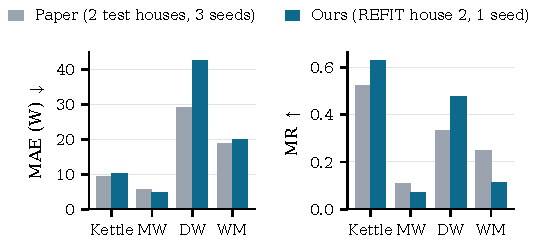
\includegraphics[width=\columnwidth]{paper_comparison}
\caption{Paper vs.\ reproduction on REFIT (MW: microwave, DW: dishwasher, WM: washing machine).}
\label{fig:paper}
\end{figure}

\subsection{All models on their test houses}
Table~\ref{tab:test} reports every model on its test house. The tumble dryer is tested on REFIT~15
because neither house~2 nor house~9 owns one. The water heater, a large resistive load, is
almost perfectly recovered (F1 \WHFone{}, SAE \WHSAE{}).

\begin{table*}[t]
\centering\footnotesize
\caption{Every model on its test house. MAE (W) and MR on the raw output; MR$_\text{pp}$, F1,
precision, recall and SAE after post-processing. R: trained on REFIT only; R+P: REFIT and Plegma.}
\label{tab:test}
% generated by paper/scripts/make_figures.py -- do not edit
\begin{tabular}{@{}llrrrrrrr@{}}
\toprule
Model & Test house & MAE & MR & MR$_\text{pp}$ & F1 & Prec. & Rec. & SAE \\
\midrule
Kettle & REFIT 2 & 10.3 & 0.631 & 0.675 & 0.835 & 0.802 & 0.872 & 0.000 \\
Microwave & REFIT 2 & 4.9 & 0.071 & 0.072 & 0.236 & 0.208 & 0.274 & 0.609 \\
Dishwasher & REFIT 2 & 42.8 & 0.475 & 0.528 & 0.802 & 0.753 & 0.857 & 0.220 \\
Washing machine (R) & REFIT 2 & 20.0 & 0.115 & 0.100 & 0.443 & 0.564 & 0.365 & 0.823 \\
Fridge (R) & REFIT 2 & 22.3 & 0.521 & 0.522 & 0.768 & 0.762 & 0.774 & 0.210 \\
Tumble dryer & REFIT 15 & 10.0 & 0.353 & 0.475 & 0.813 & 0.692 & 0.985 & 0.404 \\
Air conditioner & Plegma 101 & 89.7 & 0.426 & 0.529 & 0.809 & 0.939 & 0.711 & 0.407 \\
Water heater & Plegma 101 & 7.8 & 0.886 & 0.892 & 0.985 & 0.981 & 0.988 & 0.057 \\
Fridge (R+P) & Plegma 101 & 17.2 & 0.612 & 0.525 & 0.801 & 0.880 & 0.735 & 0.422 \\
Washing machine (R+P) & Plegma 101 & 4.7 & 0.229 & 0.329 & 0.468 & 0.409 & 0.546 & 0.161 \\
\bottomrule
\end{tabular}

\end{table*}

\subsection{Ablations}\label{sec:ablation}
Table~\ref{tab:ablation} isolates three design choices on the held-out household.

\textbf{Training data.} With the same post-processing, adding Plegma to REFIT raises the washing
machine F1 from \WMRefitOnlyFone{} to \WMFone{} and lowers its SAE from \WMRefitOnlySAE{} to
\WMSAE{}. For the fridge, the REFIT-only model reaches a \emph{higher} F1 (\FridgeRefitOnlyFone{}
vs \FridgeFone{}) but a lower MR$_\text{pp}$ (\FridgeRefitOnlyMRpp{} vs \FridgeRefitPlegmaMRpp{}).
For the fridge, Plegma thus improves the energy estimate rather than the detection.

\textbf{Threshold of cycling loads.} The F1-optimal threshold of the validation house
(\FridgeThrTunedThr{}~W, for a fridge running near 130~W) removes most cycles of the test
house's smaller fridge (about 80~W): F1 drops to \FridgeThrTunedFone{}. A fixed \FridgeThrFixedThr{}~W
threshold restores \FridgeThrFixedFone{}. Thresholds of cycling loads should not be transferred
across houses.

\textbf{Energy gain and inventory.} The gain reduces the AC SAE and the washing-machine SAE, but
slightly increases those of the fridge and the water heater. A per-appliance gain is therefore
not always beneficial. Running the dryer model on REFIT~2, which has no dryer, produces
\TDFalseKWh{}~kWh of false activations. Restricting models to the owned appliances removes them.

\begin{table*}[t]
\centering\footnotesize
\caption{Ablations on the held-out household (Plegma~101), and inventory on REFIT~2.}
\label{tab:ablation}
% generated by paper/scripts/make_figures.py -- do not edit
\begin{tabular}{@{}lllrrr@{}}
\toprule
Study & Appliance & Variant & F1 & SAE & kWh (meas./pred.) \\
\midrule
Threshold & Fridge & tuned on house 103 & 0.148 & 0.821 & 417 / 75 \\
 & Fridge & fixed 20 W & 0.801 & 0.418 & 417 / 243 \\
\addlinespace
Energy gain & Air conditioner & gain = 1 & 0.809 & 0.579 & 1446 / 608 \\
 & Water heater & gain = 1 & 0.985 & 0.033 & 638 / 617 \\
 & Fridge & gain = 1 & 0.801 & 0.298 & 417 / 293 \\
 & Washing machine & gain = 1 & 0.468 & 0.444 & 39 / 22 \\
 & Air conditioner & gain tuned on 103 & 0.809 & 0.407 & 1446 / 857 \\
 & Water heater & gain tuned on 103 & 0.985 & 0.057 & 638 / 602 \\
 & Fridge & gain tuned on 103 & 0.801 & 0.422 & 417 / 241 \\
 & Washing machine & gain tuned on 103 & 0.468 & 0.161 & 39 / 32 \\
\addlinespace
Inventory & Tumble dryer & run on house 2 & -- & -- & 0 / 120 \\
\addlinespace
Training data & Fridge & REFIT only & 0.875 & 0.454 & 417 / 228 \\
 & Washing machine & REFIT only & 0.333 & 0.270 & 39 / 49 \\
 & Fridge & REFIT + Plegma & 0.801 & 0.422 & 417 / 241 \\
 & Washing machine & REFIT + Plegma & 0.468 & 0.161 & 39 / 32 \\
\bottomrule
\end{tabular}

\end{table*}

% =============================================================================================
\section{Case Study: One Household}\label{sec:house}
The backend serves a single household, Plegma~101, so that every view relies on one consistent
data source. We chose it because it is held out from every model and has the longest record
(\HouseDays{} valid days, \HouseMissing\% missing minutes). It also owns the four appliances most
relevant to Vietnamese homes, which account for \HouseMetered\% of its \HouseKWh{}~kWh.
Thresholds and gains come from Plegma~103. The mean F1 over the four appliances is
\HouseMeanFone{} (Table~\ref{tab:house}).

\begin{table*}[t]
\centering\footnotesize
\caption{Household Plegma~101 (15 Jul 2022 -- 30 Sep 2023), after post-processing.}
\label{tab:house}
% generated by paper/scripts/make_figures.py -- do not edit
\begin{tabular}{@{}lrrrrrrrr@{}}
\toprule
Appliance & F1 & Prec. & Rec. & MAE & RMSE & SAE & NDE & kWh (meas./pred.) \\
\midrule
Air conditioner & 0.809 & 0.939 & 0.711 & 73.2 & 246.5 & 0.407 & 0.313 & 1446 / 857 \\
Water heater & 0.985 & 0.981 & 0.988 & 7.0 & 88.1 & 0.057 & 0.030 & 638 / 602 \\
Fridge & 0.801 & 0.880 & 0.735 & 20.4 & 32.6 & 0.422 & 0.319 & 417 / 241 \\
Washing machine & 0.468 & 0.409 & 0.546 & 3.5 & 65.0 & 0.161 & 0.632 & 39 / 32 \\
\bottomrule
\end{tabular}

\end{table*}

\textbf{Consumption mix.} The models recover \HouseFound\% of the metered appliances' energy
(Fig.~\ref{fig:mix}). The water heater and the washing machine are close to their measured
shares. The AC share falls from \ACTrueShare\% to \ACPredShare\% and the fridge share from
\FridgeTrueShare\% to \FridgePredShare\%. The missed energy is attributed to ``Other'', which
grows from \OtherTrueShare\% to \OtherPredShare\%.

\begin{figure}[t]
\centering
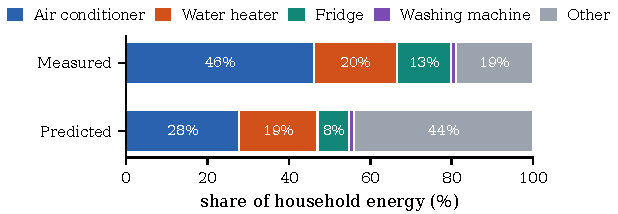
\includegraphics[width=\columnwidth]{house101_mix}
\caption{Share of household energy, measured vs.\ predicted (Plegma~101).}
\label{fig:mix}
\end{figure}

\textbf{Air conditioner.} Detection is reliable (precision \ACPrec{}), and the energy depends on
the season (Fig.~\ref{fig:monthly}, Table~\ref{tab:quarterly}). In July 2023 the model finds
\ACJulPred{} of \ACJulTrue{}~kWh (\ACJulPct\%), but in January 2023 it finds \ACJanPred{} of
\ACJanTrue{}~kWh (\ACJanPct\%). The quarterly F1 ranges from \ACQfourF{} (Q4/2022) to
\ACQthreeF{} (Q3/2023). In winter the units run as heat pumps, whereas most training activations
are in cooling mode, and PRECON contains cooling only. For a cooling-dominated climate such as
Vietnam's, the summer figures are the relevant ones. Daily AC energy correlates at $r=0.92$
with the measurement (Fig.~\ref{fig:scatter}).

\begin{figure*}[t]
\centering
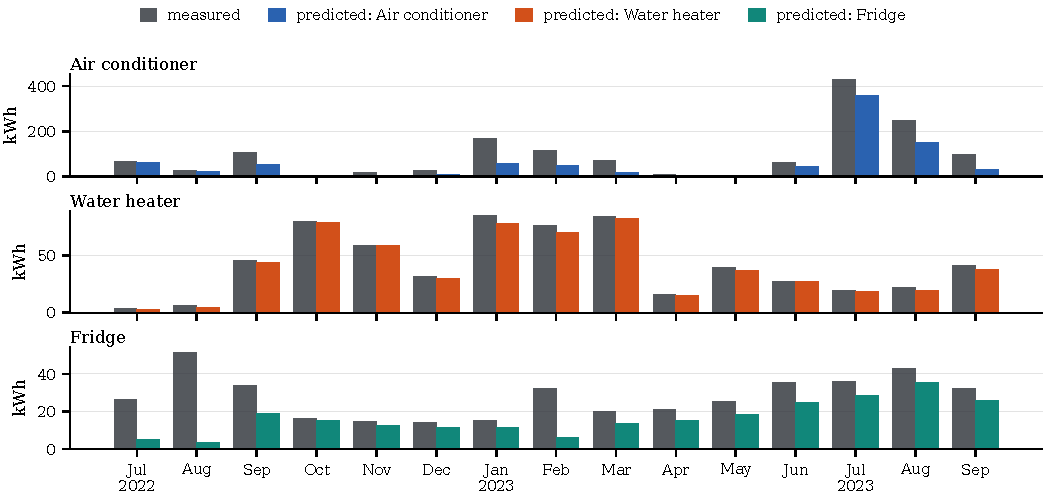
\includegraphics[width=\textwidth]{house101_monthly}
\caption{Monthly energy per appliance, measured vs.\ predicted (July 2022 covers 15.5 days).}
\label{fig:monthly}
\end{figure*}

\begin{table}[t]
\centering\footnotesize
\caption{Quarterly F1 on Plegma~101 (Q3/2022 starts on 15 July).}
\label{tab:quarterly}
% generated by paper/scripts/make_figures.py -- do not edit
\begin{tabular}{@{}lrrrrr@{}}
\toprule
Appliance & Q3/2022 & Q4/2022 & Q1/2023 & Q2/2023 & Q3/2023 \\
\midrule
Air conditioner & 0.784 & 0.476 & 0.699 & 0.688 & 0.874 \\
Water heater & 0.985 & 0.981 & 0.987 & 0.978 & 0.969 \\
Fridge & 0.497 & 0.863 & 0.697 & 0.957 & 0.916 \\
Washing machine & 0.478 & 0.390 & 0.597 & 0.488 & 0.260 \\
\bottomrule
\end{tabular}

\end{table}

\textbf{Fridge.} On \FridgeConstDays{} days (July--September 2022 and February 2023) the fridge
draws about \FridgeConstW{}~W every minute of the day, with no compressor cycling. A constant
load has no switching edge in the aggregate and is indistinguishable from the base load, so no
NILM model can attribute it. These days form the outlier cluster of Fig.~\ref{fig:scatter} and
the monthly deficit of Fig.~\ref{fig:monthly}. Without them, the fridge F1 is \FridgeExclFone{},
the SAE \FridgeExclSAE{}, and the daily correlation rises from \FridgeDailyRall{} to
\FridgeDailyRexcl{}. The constant draw may come from a defrost fault or from another load sharing
the plug; the dataset does not tell.

\begin{figure*}[t]
\centering
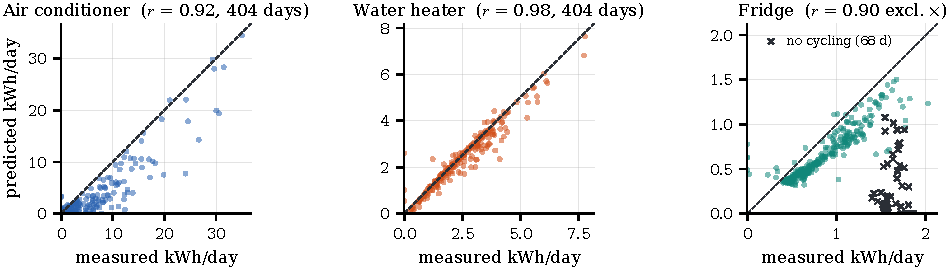
\includegraphics[width=\textwidth]{house101_daily_scatter}
\caption{Daily energy, measured vs.\ predicted (days with $\geq$90\% of the minutes). Crosses:
fridge days without compressor cycling, excluded from $r$.}
\label{fig:scatter}
\end{figure*}

\textbf{One day.} Fig.~\ref{fig:day} shows 12 July 2023. The AC cycles and the single
water-heater activation are tracked, with the AC level slightly under-estimated. After a two-hour
gap in the data, the AC is missed for about 70~minutes, because the windows that overlap the gap
lack context. Short gaps should be filled before calling the service.

\begin{figure}[t]
\centering
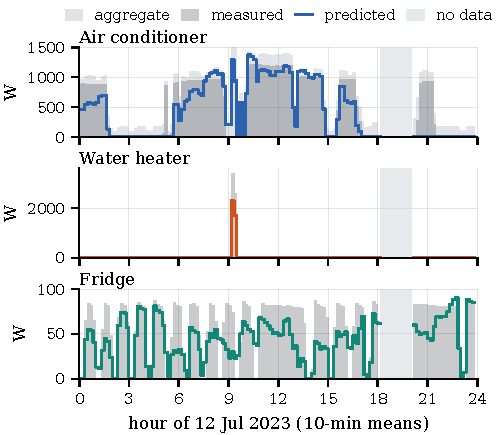
\includegraphics[width=\columnwidth]{house101_day}
\caption{12 July 2023, 10-min means. Grey band: missing data.}
\label{fig:day}
\end{figure}

\textbf{Washing machine.} It uses 1\% of the household energy. The energy error is small
(SAE \WMSAE{}), but individual cycles are often confused with other loads of similar power
(precision \WMPrec{}).

% =============================================================================================
\section{Limitations}
These results use one seed and a single test and validation house per appliance, so they vary with
the house chosen. No training house is Vietnamese: climate, AC types (inverter vs.\ fixed-speed) and
usage habits only approximate the target. The AC level is under-estimated, especially in heating
mode, and a single annual gain cannot correct a seasonal bias. PRECON carries no licence statement,
so we use it for research only.

\section{Conclusion}
NILMFormer reproduces on REFIT with mixed results relative to the paper: two of four appliances
improve in MR. Harmonising Plegma and PRECON into the REFIT layout lets the same pipeline train
models for air conditioners and water heaters. On an unseen household these models reach an F1 of
\ACFone{} and \WHFone{} respectively. The next step is a small set of sub-metered Vietnamese
households to fine-tune the AC model. Promising directions are longer windows for long AC cycles,
an ON-weighted loss against level shrinkage, and seed ensembles.

\section*{Reproducibility}
Code: \texttt{nilmformer-experiment/} (pipeline, converter, post-processing). The command
\texttt{make paper-data paper-figures paper} regenerates every table, figure and number of this
paper from the trained models. \texttt{make validate} runs a 13-step smoke test of the chain.

\bibliographystyle{IEEEtran}
\bibliography{refs}

\end{document}
